\documentclass[a4paper, 12pt]{extarticle}

% Поля
%--------------------------------------
\usepackage{geometry}
\geometry{a4paper,tmargin=2cm,bmargin=2cm,lmargin=3cm,rmargin=1cm}
%--------------------------------------


%Russian-specific packages
%--------------------------------------
\usepackage[T2A]{fontenc}
\usepackage[utf8]{inputenc} 
\usepackage[english, main=russian]{babel}
%--------------------------------------

\usepackage{textcomp}

% Красная строка
%--------------------------------------
\usepackage{indentfirst}               
%--------------------------------------             


%Graphics
%--------------------------------------
\usepackage{graphicx}
\graphicspath{ {./images/} }
\usepackage{wrapfig}
\usepackage{minted}
%--------------------------------------

% Полуторный интервал
%--------------------------------------
\linespread{1.3}                    
%--------------------------------------

%Выравнивание и переносы
%--------------------------------------
% Избавляемся от переполнений
\sloppy
% Запрещаем разрыв страницы после первой строки абзаца
\clubpenalty=10000
% Запрещаем разрыв страницы после последней строки абзаца
\widowpenalty=10000
%--------------------------------------

%Списки
\usepackage{enumitem}

%Подписи
\usepackage{caption} 

%Гиперссылки
\usepackage{hyperref}

\hypersetup {
	unicode=true
}

%Рисунки
%--------------------------------------
\DeclareCaptionLabelSeparator*{emdash}{~--- }
\captionsetup[figure]{labelsep=emdash,font=onehalfspacing,position=bottom}
%--------------------------------------

\usepackage{tempora}
\usepackage{amsmath}
\usepackage{color}
\usepackage{listings}
\lstset{
  belowcaptionskip=1\baselineskip,
  breaklines=true,
  frame=L,
  xleftmargin=\parindent,
  language=Python,
  showstringspaces=false,
  basicstyle=\footnotesize\ttfamily,
  keywordstyle=\bfseries\color{blue},
  commentstyle=\itshape\color{purple},
  identifierstyle=\color{black},
  stringstyle=\color{red},
}

%--------------------------------------
%			НАЧАЛО ДОКУМЕНТА
%--------------------------------------

\begin{document}

%--------------------------------------
%			ТИТУЛЬНЫЙ ЛИСТ
%--------------------------------------
\begin{titlepage}
\thispagestyle{empty}
\newpage


%Шапка титульного листа
%--------------------------------------
\vspace*{-30 pt}
\hspace{-65pt}
\begin{minipage}{0.3\textwidth}
\hspace*{-20pt}\centering

\includegraphics[width=60pt]{emblem}
\end{minipage}
\begin{minipage}{0.67\textwidth}\small \textbf{
\vspace*{-0.7ex}
\hspace*{-6pt}\centerline{Министерство науки и высшего образования Российской Федерации}
\vspace*{-0.7ex}
\centerline{Федеральное государственное бюджетное образовательное учреждение }
\vspace*{-0.7ex}
\centerline{высшего образования}
\vspace*{-0.7ex}
\centerline{<<Московский государственный технический университет}
\vspace*{-0.7ex}
\centerline{имени Н.Э. Баумана}
\vspace*{-0.7ex}
\centerline{(национальный исследовательский университет)>>}
\vspace*{-0.7ex}
\centerline{(МГТУ им. Н.Э. Баумана)}}
\end{minipage}
%--------------------------------------

\vspace{10pt}
\hspace{-35pt} \noindent \small ФАКУЛЬТЕТ\hspace{80pt} <<Информатика и системы управления>>

\vspace*{-16pt}
\hspace{47pt}\rule{0.83\textwidth}{0.4pt}

\vspace{0.5ex}
\hspace{-35pt} \noindent \small КАФЕДРА\hspace{50pt} <<Теоретическая информатика и компьютерные технологии>>

\vspace*{-16pt}
\hspace{30pt}\rule{0.866\textwidth}{0.4pt}
  
\vspace{6em}

\begin{center}
\Large {\bf Лабораторная работа № 2} \\ 
\large {\bf по курсу <<Языки и методы программирования>>} \\ 
\large «Разработка простейшего класса на языке Java.» \\
\large <<Вариант 18>>
\end{center}\normalsize

\vspace{15em}


\begin{flushright}
  {Студент группы ИУ9-21Б: Пенкин А. Д.\hspace*{15pt} \\
  \vspace{2ex}
  Преподаватель: Посевин Д. П.\hspace*{15pt}}
\end{flushright}

\bigskip

\vfill
 \vspace{7em}

\begin{center}
\textsl{Москва 2023}
\end{center}
\end{titlepage}
%--------------------------------------
%		КОНЕЦ ТИТУЛЬНОГО ЛИСТА
%--------------------------------------

\renewcommand{\ttdefault}{pcr}

\setlength{\tabcolsep}{3pt}
\newpage
\setcounter{page}{2}

\section{Цель}\label{Sect::task}
\par
Целью данной работы является изучение базовых возможностей языка Java.
\section{Условие}
Выполнение лабораторной работы заключается в составлении на языке Java класса, представляющего матрицу расстояний между всеми парами из n городов с операцией вычисления длины пути, заданного последовательностью посещаемых городов. И реализация тесирующего его файла.
\section{Код решения}
1. Cities.java
\begin{minted}{java}
public class Cities {
    private int n;
    private int [][] roads;
    public Cities(int k){
        roads = new int[k][k];
        for (int i = 0; i < k; i++){
            for (int j = 0; j < k; j++){
                if (i == j)
                    this.roads[i][j] = 0;
                else
                    this.roads[i][j] = -1;
            }
        }
        n = k;
    }
    public void setRoad(int a, int b, int l){
        System.out.println("дорога из *" + a + "* в *" +
                b +"* равна: " + l);
        this.roads[a][b] = l;
        this.roads[b][a] = l;
    }
    public void outMatrix(){
        for (int i = 0; i < n; i++){
            for (int j = 0; j < n; j++) {
                System.out.print(roads[i][j] + " ");
            }
            System.out.println();
        }
    }
    public int path(int[] nums){
        int sum = 0;
        System.out.print("пройдём по пути городов под номерами: ");
        for (int i = 0; i < nums.length - 1; i++){
            System.out.print(nums[i] + "->");
        }
        System.out.println(nums[nums.length - 1]);
        for (int i = 0; i < nums.length - 1; i++){
            if (this.roads[nums[i]][nums[i + 1]] < 0) {
                System.out.print("дороги из города *"+nums[i]);
                System.out.println("* в город *"+nums[i + 1]+"* не существует,");
                System.out.print("пожалуйста, создайте дорогу или ");
                System.out.println("выберите другую последовательность городов.");
                return -1;
            }
            sum += this.roads[nums[i]][nums[i + 1]];
        }
        return sum;
    }
    public int getRoad(int a, int b){
        return roads[a][b];
    }
}
\end{minted}
2. Test.java
\begin{minted}{java}
public class Test {
    public static void main(String[] args) {
        int n = 5;
        System.out.println("пусть количество городов: 5");
        Cities loc1 = new Cities(n);
        System.out.println();
        System.out.println("начальная матрица:");
        loc1.outMatrix();
        System.out.println();
        System.out.println("запишем некоторые дороги");
        loc1.setRoad(1, 2, 25);
        loc1.setRoad(1, 0, 10);
        loc1.setRoad(1, 4, 65);
        loc1.setRoad(3, 4, 3);
        loc1.setRoad(0, 2, 1);
        loc1.setRoad(2, 3, 12);
        System.out.println();
        System.out.println("новая матрица городов: ");
        loc1.outMatrix();
        System.out.println();
        int [] a = new int[] {0, 3, 2, 3};
        int [] b = new int[] {0, 1, 2, 3};
        int path1 = loc1.path(a);
        if (path1 > 0)
            System.out.println("этот путь равен: " + path1);
        System.out.println();
        int path2 = loc1.path(b);
        if (path2 > 0)
            System.out.println("этот путь равен: " + path2);
    }

}
\end{minted}


\section{Результаты работы программы}
\begin{figure}[H]
    \centering
    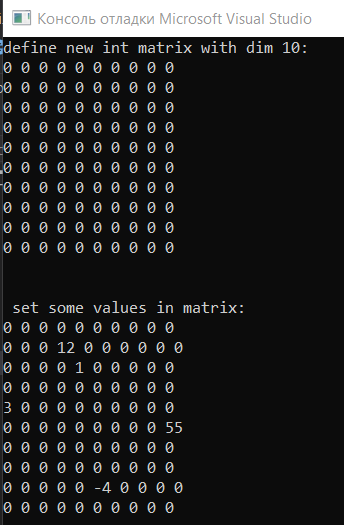
\includegraphics[width=300pt]{Test.png}
    \caption{создание обЪекта матрицы расстояний}
    \label{fig:my_label}
\end{figure}

\begin{figure}[H]
    \centering
    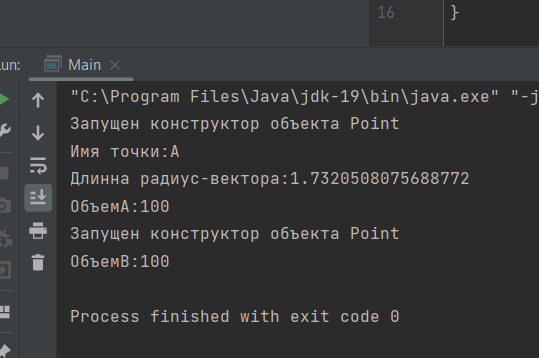
\includegraphics[width=300pt]{Test1.png}
    \caption{создание дорог, изменение матрицы}
    \label{fig:my_label}
\end{figure}

\begin{figure}[H]
    \centering
    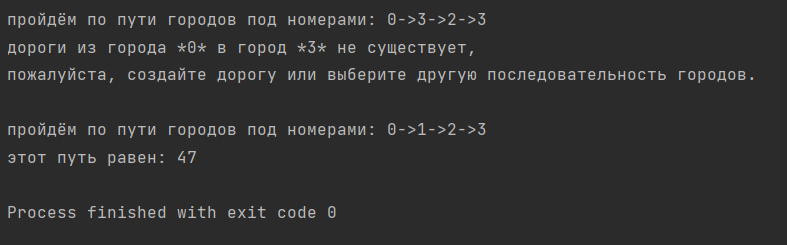
\includegraphics[width=\linewidth]{Test2.png}
    \caption{подсчёт пути}
    \label{fig:my_label}
\end{figure}


\end{document}